%%=============================================================================
%% Interviews
%%=============================================================================

\chapter{Interviews}
\label{ch:interviews}

Zoals in het vorig hoofdstuk vermeld worden er drie experts uit het vakgebied geïnterviewd. Het vinden van de juiste datum en plaats om deze interviews te doen ging steeds vlot, de geïnterviewden werkten zeer goed samen op dit vlak. Per geïnterviewde is er een hoofdstuk aangemaakt, met daarin een korte inleiding over de expert zelf en achteraf de antwoorden op de vragen die gesteld zijn.

\section{Interview Filip Polfiet}
\label{sec:interview-filip}

Filip is een Digital Marketeer met vele jaren ervaring in digitale marketing, community management, copywriting, IT projecten leiden (voornamelijk web-gebaseerde applicaties), ontwerpen van creatieve advertenties en ook het ontwerpen en onderhouden van websites. 

Deze jaren ervaring zijn gestart met een grondige basis van drie diploma's. Hij heeft eerst zijn diploma journalistiek behaald, daarna politieke en sociale wetenschappen en als laatste een master in conflict en development. Na deze vele jaren studeren zag Filip de opkomst van websites en hij had hier veel interesse in. Daarom heeft Filip bijgeschoold over webtechnologieën en in eerste instantie hoe je een website maakt. 

Dit gaat van Wordpress websites tot de achterliggende architectuur en HTML, CSS, JS, ... en ook verder over SEO, SEA en het opvangen van alle data in Google Analytics en nog zoveel meer. 

Filip is nu freelance consultant voor een digital agency in Anderlecht en een start-up van Belfius genaamd Jaimy. Voordien heeft Filip gewerkt voor Plan International België, waar hij een groot IT project heeft opgestart. Bij Handicap International België heeft hij ook verschillende jaren in een leidende functie de digitale marketing verzorgd. Als consultant voor Woody werkte hij recent aan de digitale marketing van het pyjamabedrijf. Naast deze technische -en marketingskills bezit hij ook een goed inzicht in het creatieve deel van marketing zoals het maken van posters, filmpjes, geluidsbewerking enzovoort.

\textbf{Heeft u al van growth hacking gehoord?}
	
Filip kent growth hacking al, hij beschrijft het als een voornamelijk creatieve marketing strategie die veel impact heeft met weinig budget. De lijn tussen growth hacking en guerrillamarketing blijft echter wel vaag, want het zijn twee marketing strategieën die veel op elkaar lijken. 

Wat jammer genoeg vaak gebeurt bij dit soort marketingstrategieën is dat het geforceerd over komt. Andere bedrijven proberen dezelfde growth hack uit te voeren als een succesvol bedrijf deed, maar dat werkt dus bijna nooit.

\textbf{Hoe past u dit toe binnen uw bedrijf?}
	
Filip werkte tot enkele maanden geleden voor Woody, een Gents pyjamabedrijf. Het is een vrij klassiek bedrijf dat geen super opvallende marketing nodig heeft. Het was dus niet noodzakelijk om iets als growth hacking toe te passen bij dit type bedrijf, het was namelijk ook niet de vraag van hen uit. Woody wou vooral aan brand awareness doen, dat wil zeggen dat men er voor gaat zorgen dat mensen Woody leren kennen als merk. 

Indien Filip growth hacking zou toepassen zou hij dat ook niet enkel via Facebook Ads doen (want dat is wat Filip doet voor Woody). Jammer genoeg is het ook iets dat veel bedrijven niet durven. Growth hacking is ook durven, dingen uitproberen, experimenteren en falen. Dat is wat bij er volgens Filip bij veel (grote) bedrijven ontbreekt.
	
\textbf{Wat zijn uw belangrijkste resources voor de groei van een bedrijf? Steunt u op AdWords, Facebook Ads etc?}
	
Groei is een en-en-verhaal. Er moeten meerdere kanalen gebruikt worden zoals E-mail, Facebook en Instagram advertenties (de laatste twee gebeuren via het Facebook Ads platform), Google ads (wat minder belangrijk is omdat niet per sé creatief is, het werkt eerder ondersteunend). Voor Filip is Facebook Ads het beste platform, het is een goede tool omdat onderzoek doet blijken dat de gemiddelde belg of Europeaan minstens 30 minuten per dag aan Facebook besteed.

\textbf{Hoe ging u in het begin van uw carrière om met (community)-groei van een bedrijf en hoe doet u dat nu? Wat is er veranderd in die tijd? Wat heeft u geleerd?}
	
Toen Filip begon bestond er geen sociale media en al zeker geen advertenties op sociale media. De websites bestonden nog maar net en waren geen ``big deal``. 
Vandaag de dag zijn er zoveel verschillende kanalen om mensen te bereiken, zoals sociale media en talloze andere websites. Men kan spreken van een \emph{information overload}. 

In het veld van marketing heeft het heel veel voordelen, de toegang tot al deze kanalen om klanten te vinden. Bovendien zijn al deze kanalen heel meetbaar, er kan eenvoudig worden nagegaan of er efficiënt gewerkt wordt.
		
\textbf{Heeft u ervaring met Zero Budget Marketing? Wat is hierbij het belangrijkste onderdeel van marketing?}
	
	Het belangrijkste is om heel creatief te zijn. Je moet alle kanalen gebruiken die beschikbaar zijn. Je moet je verspreiden via al die kanalen, en zo'n dingen zijn zeer moeilijk met weinig budget, maar zeker mogelijk, mits goede brainstorm sessies en een goed idee. 
	
	Uit eigen ervaring bij Plan België: op Pukkelpop wou Plan België een actie doen rond kind huwelijken. Initieel wouden ze flyers uitdelen op het festival, maar Filip wou dit origineler aanpakken. Het moet verder gaan dan enkel flyers uitdelen, daarmee bereik je niet veel bij de doelgroep van 15-25 jarigen. Dus Filip bedacht het idee van een stand waar koppels of vrienden zichzelf konden ``uithuwelijken``. Hier konden ze een ludieke foto nemen en tijdens het proces of achteraf kregen ze een uitleg dat deze leuke stand eigenlijk wel meer betekenis had dan enkel een toffe foto maken met je vrienden. Er zat veel meer achter en bracht zo aandacht bij de jongeren dat er in vele landen wel effectief een probleem is dat jonge meisjes worden uitgehuwelijkt aan een oudere man waar ze helemaal niet mee willen samen zijn. Filip heeft hierbij de volledige uitwerking verzorgd, van idee tot uitwerking van de stand en bijstand van het IT-team. Want dit maakt het zero budget marketing idee ook wel growth hack, doordat IT, marketing en creatieve ontwerpers samenkomen. Aan deze stand was een hele technische kant verbonden waarbij je je e-mailadres kon invullen en wanneer je dan een foto nam kreeg je die foto opgestuurd naar je e-mailadres. Ook was er een iPad voorzien waarmee je een foto kon nemen en deze eenvoudig uploaden op je social media.
	
	Een tweede ervaring, ook bij Plan België, ging over een simpele social media post dat inspeelde op een in die tijd populaire trend: ``Keep calm and ****``. Filip speelde hier op in tijdens moederdag, waar hij de briefing kreeg om een leuke post te maken voor sociale media in verband met sociale media en moederdag. Hij schreef een eenvoudige post met ``Keep calm and don't forget moederkesdag``. Enkel de manier waarop ``moederkersdag`` werd geschreven zorgde voor verschillende reacties en mensen die reageerde op deze post, elkaar tagde enz... Dit toont aan hoe belangrijke de juiste copywriting is en een combinatie van een originele post die inspeelt op de huidige trends.
	
	Een derde ervaring bij Plan België is een groot IT project waarbij ze een eigen crowd funding platform hebben kunnen starten voor vrij weinig geld, ongeveer 25.000 euro. Hier kon iedereen een eigen project starten met een foto en wat tekst waarbij ze hun reden voor geldinzameling verkondigden. Dit kan bijvoorbeeld een huwelijksjubileum zijn, waar de twee getrouwde geen cadeaus willen, maar enkel een goed doel steunen. Dat kan dan via het online platform waar ze enkel een link moeten delen. Daardoor moet het niet meer via hun eigen bankrekening gebeuren. Deze link kan ook verder op sociale media gedeeld worden en zorgt dus voor het belangrijke onderdeel van marketing: referral.
	
	Het laatste voorbeeld is bij Woody, het pyjama bedrijf in Gent: je moet steeds de realiteit en actualiteit in het oog houden. Je moet als marketeer heel bewust zijn van de feiten en deze in iets positief kunnen omzetten. Bijvoorbeeld: de website van Woody lag tijdens de Sint-periode plat, door een technisch probleem. Als digital marketeer kan je hier heel leuk mee omgaan, zoals Filip deed, met een ludieke post. Filip heeft een foto van de Sint, die iemand voor Woody had gemaakt, bewerkt met een draad, waar de Sint over viel. Hierbij werd de tekst geplaatst ``De sint struikelde over de draad en heeft perongeluk de website neergehaald, we doen ons best om dit op te lossen!``. Door deze leuke post is iedereen op de hoogte en toch niet boos op het bedrijf.
	
\textbf{Waaruit bestaat een ideaal marketing team volgens u? In verhouding: hoeveel copywriters, digital marketeers, programmeurs, creatief ontwerpers, enz.?}
	
	De basis is volgens Filip sowieso: een copywriter, grafisch ontwerper en een programmeur/analytisch denker dit met de cijfers en de code kan werken. Hierbij hoort steeds ook een out-of-the-box denker of een gek persoon. Deze kan 1 van de andere functies delen, zoals copywriter.	
	
	Verschillende personen zijn belangrijk, natuurlijk is dit afhankelijk van de grootte van het bedrijf. Er mag geen negatief persoon tussen zitten die niet open staat voor andere ideeën tijdens de brainstorm sessie, want zo creëer je een negatieve sfeer. Je mag tijdens zo'n sessies niet te realistisch zijn; ``dit kan niet want x en y`` is niet wat je wil. Je kan moeilijk op een goed, creatief idee komen in een vergadering met 20 mensen waarvan enkele accountancy en managers dit te veel met cijfers bezig zijn. Je moet los van de cijfers, los van het budget kunnen ``freewheelen`` en het volledige tegenovergestelde durven denken dan dat wat er gepland is. Dit kan moeilijk om een voorafgedefinïeerde tijdspanne, zoals 4 uur in de namiddag. Zo'n ideeën hebben tijd nodig.
	
\textbf{Hoe belangrijk is viraal gaan voor een bedrijf? Is dit volgens u waar iedere marketeer, zoals uzelf, naar streeft? Of is het een specifiek doel dat op de juiste moment wordt achtervolgd?}
	
Dit gaat natuurlijk niet altijd en is iets dat moeilijk is. Het kan bijvoorbeeld 1 keer per jaar, maar het is niet iets dat consistent kan gebeuren. De post op sociale media moet bijvoorbeeld heel creatief, goed gevonden en origineel zijn voordat deze viraal kan gaan. De creativiteit staat centraal hierbij. Natuurlijk hopen veel digital marketeers dat hun post viraal gaat, maar dit is natuurlijk zelden het geval. Bedrijven moeten hier ook niet op focussen, goede content is beter dan geforceerde content die bedoeld is om viraal te gaan.

Een virale post kan van alles zijn en is vaak toevallig. Het kan een goed getimede gif zijn van een sociale media community manager of een leuke reactie op Twitter of een goede post die op de juiste moment is gepost in de juiste context, ... Soms lijken deze reacties of posts heel spontaan, maar is er door de bedrijven wel goed over nagedacht.
	
\textbf{Bij growth hacking spreekt men vaak over 2 à 3 belangrijke onderdelen: Creativiteit, Experimenteren/Analyseren van data en tot slot het Automatiseren en toepassen op technisch vlak. Ook bent u niet bewust bezig met growth hacking, deze onderdelen komen ook aan bod bij traditionele of digitale marketing.}
\begin{enumerate}[label*=\arabic*.]
	\item \textbf{Creativiteit: Hoe gaat u om met het creatieve proces van marketing? Bijvoorbeeld: Zijn hier brainstorm sessies voorzien? Heeft u creatieve ontwerpers die helpen?}
	
	Volgens Filip is het de basis van alles. Je moet eerst veel nadenken voordat je begint met ontwikkeling van het technische aspect van je idee. De start is steeds een goed en creatief idee. Het is belangrijk om hier voldoende tijd aan te spenderen voordat je verder gaat.
	
	\item \textbf{Data: Welke tools gebruikt u om informatie te verzamelen over uw doelpubliek? Welke tool is het belangrijkst en waarom?}
	
	Google Analytics
	
	\item \textbf{Automatiseren: Welke rol speelt IT of het IT-team bij marketing volgens u? }
	
	Het IT team speelt een heel belangrijke rol, maar daar loopt het vaak fout. De communicatie en vlotte werking is cruciaal, het is vaak moeilijk om iets gedaan te krijgen in een IT team. Hiervoor is goede communicatie belangrijk.
	
	De laatste 2 punten, Data en automatiseren zijn bijkomend en eerder logisch, terwijl het eerste punt, de creativiteit het belangrijkste en moeilijkste proces is van de 3.
	
\end{enumerate}
\textbf{In de termen van growth hacking: is er een experiment dat u al lang wil uitvoeren, maar nog geen middelen heeft voor gehad?}

Een nieuw concept, een eigen start-up waar alles mogelijk is. Niet per sé iets heel concreet, maar een bedrijf waar men durft risico's nemen, want het risico is klein, want het kost niet veel.

\textbf{Growth hacking is vooral gekend bij online start-ups zoals Airbnb, Hotmail en Dropbox. Veranderd er volgens u veel bij growth hacking wanneer het niet meer gaat om een online bedrijf, maar wel een start-up met een fysiek product, zoals de krekelreep van Kriket?}

Het is zeker mogelijk, want het is een nieuw, origineel en creatief product. Het belangrijkste wordt een originele invalshoek vinden. Voor Kriket is het belangrijk om in te spelen op de actualiteit, zoals het klimaat. Ze moeten zoeken naar wie er geïnteresseerd is in een Kriket-bar. Wie durft zo'n krekelreep op te eten? Dat moeten ze uitzoeken. Een voorbeeld kan zijn; de ``Kriket challenge``. Hier kan men inspelen op de brug dat de meeste belgen maken van nog nooit insecten gegeten te hebben naar een Kriket-bar. Na de krekelreep is het ijs vaak gebroken en durft men andere insect-gebaseerde gerechten te eten. Rond het concept van de challenge kunnen enkele leuke video's gemaakt worden die in een marketing campagne gebruikt kunnen worden. De video's kunnen de extreme emoties weergeven die mensen hebben bij hun eerste bijt van een krekelreep met achteraf de brede glimlach waaruit blijkt dat het echt lekker is. En dat met geen schrik moest hebben voor de krekels in de krekelreep. ``Durft gij het aan?`` zou een mogelijke manier zijn om de campagne te nemen. Waar willekeurige mensen worden uitgedaagd om de krekelreep te proberen.

\textbf{Wat denk je van growth hacking?}

Goed als klein bedrijf dat zoekt naar snelle groei. Het houdt in dat je veel risico neemt en heel creatief bent met je campagne of growth hack.
	

\section{Interview Damien Querbes}
\label{sec:interview-damien}

Damien Querbes, opgegroeid in Parijs, heeft 2 masters behaald, in ``Corporate Finance`` en ``Entrepreneurship``. Na deze studies heeft hij 3 stages gedaan bij verschillende bedrijven. Bij zijn eerste stage lag de focus op financiën, de tweede stage was eerder ondernemen en de laatste stage was in een start-up. 

Tijdens die laatste stage is Damien geheadhunt en werd hij de rechterhand van 2 co-founders van Europecar en Ubeeqo. De 2 bedrijven werden toen samengevoegd, dus ook de teams en de bedrijfsculturen. Hij heeft veel gewerkt in Brussel, Parijs en Berlijn, in het laatst vermelde land heeft hij een opleiding gekregen van een collega, die nu nog steeds een goede vriend is van hem. Zijn collega heeft hem opgeleid in digital marketing en toen heeft hij de smaak van marketing te pakken gekregen. Hij heeft geholpen met een nieuw merk te gaan rebranden. Een bedrijf van B2B naar B2C omzetten, prijzen bepalen en andere strategische beslissingen nemen.

Naast deze enorme opgave begon Damien meer en meer interesse te krijgen in digitale marketing en vooral de data die er allemaal bij komt kijken. Daarom is hij beginnen leren programmeren, zo kon hij nauw in contact staan met het IT team en het proces begrijpen waar ze door gaan. Hij kreeg de titel ``Marketing Architect``, waarbij het hele IT-deel van het marketing-team moest managen. De infrastructuur van alle tools die gebruikt worden tot de heel technische samenwerking tussen deze tools.

Nu heeft hij besloten om een nieuwe uitdaging aan te gaan bij Jaimy, als Head of Marketing probeert hij het online platform Jaimy aan de man te brengen.

\textbf{Heeft u al van growth hacking gehoord? Zo ja: hoe past u dit toe binnen uw bedrijf?}
	
Ja, Damien kent growth hacking via zijn carrière die hij heeft opgebouwd. Hij heeft de term growth hacking zien groeien, de hype zien stijgen en begrijpt het concept dus goed.

Hij gebruikt het niet, hij gelooft niet in Growth hacking. Het is een short-term strategie. Damien verkiest een long-term strategie waarbij je uiteindelijk meer bereikt. Desondanks zijn er wel enkele growth hacks die hij gebruikt en aanraadt, maar dit betekent niet dat hij growth hacking een goede marketingstrategie vindt op zich. 

De growth hack die Damien recent heeft toegepast is het toevoegen van ``?location=Brussel`` aan de link vanuit de advertenties. In de Google en Facebook advertentie platformen kan je dynamisch de stad toevoegen. Met deze link voelt de website veel persoonlijker aan, de titel wordt aangepast naar jouw locatie en uit de cijfers is er bewijs dat dit de conversies verhoogd.

\begin{figure}[h!]
	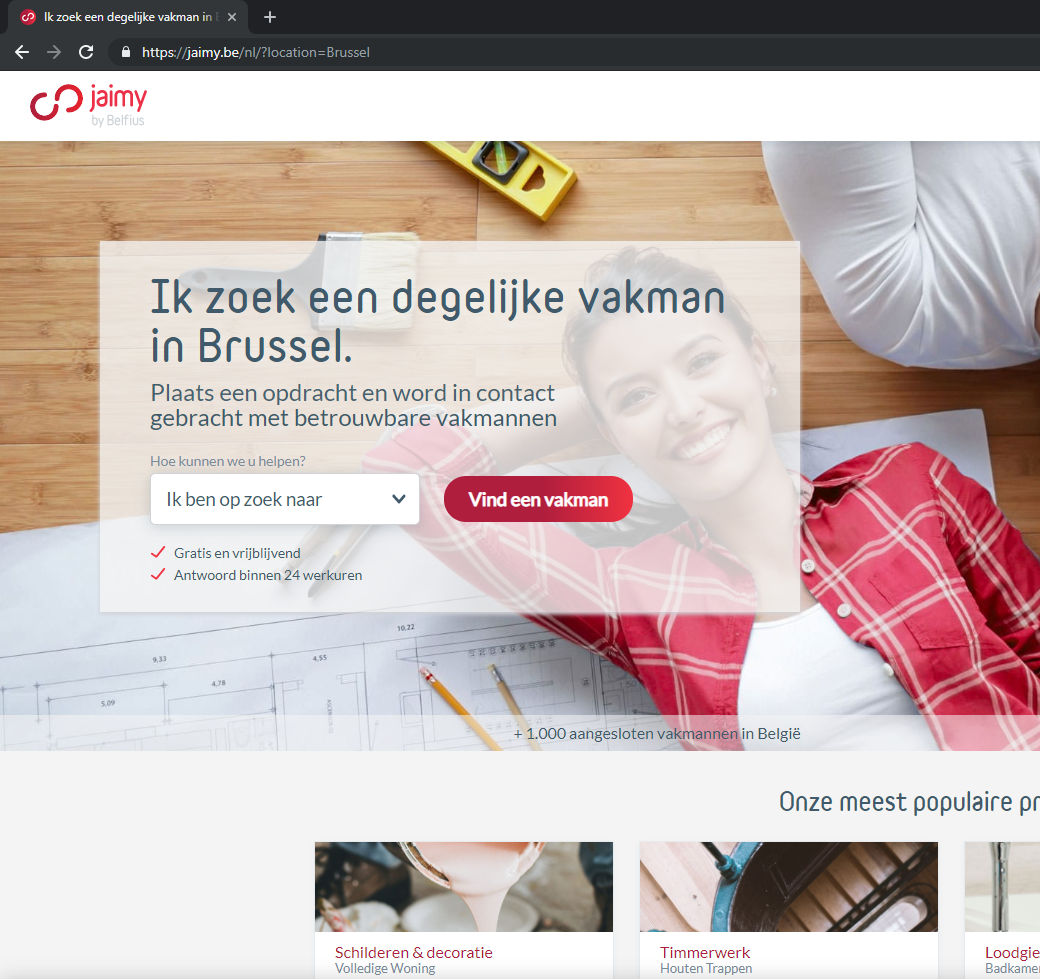
\includegraphics[width=\linewidth]{img/location-growth-hack.png}
	\caption{De simpele growth hack die Damien heeft toegepast op de website van Jaimy (\href{https://jaimy.be/nl/?location=Brussel}{https://jaimy.be/nl/?location=Brussel})}
	\label{fig:fantalism}
\end{figure}
	
\textbf{Wat zijn uw belangrijkste resources voor de groei van een bedrijf? Steunt u op AdWords, Facebook Ads etc?}
	
Aanvullende op de vorige vraag, goede long-term strategie die Damien nu toepast op Jaimy is het bouwen van de fundamenten van je merk. Dit doet hij via Google Adwords en Facebook Ads en hij baseert zijn advertenties op de basisdocumenten die bij de opstart van Jaimy zijn gemaakt. Dit zijn de missie, de visie, de USP's (Unique Selling Propositions); de meerwaarden dat de klanten uit Jaimy kunnen halen, het brandbook of huisstijlregelmentenboek (met de huisstijl, slogan, tone of voice, enz...) en de elevator pitch. 

Na het pushen van veel advertenties is het doel om de marketing langzaam aan over te laten gaan naar mond tot mond reclame. Dan zal er minder marketing aan deze kanalen gespendeerd worden. 

\textbf{Heeft u ervaring met Zero Budget Marketing? Wat is hierbij het belangrijkste onderdeel van marketing?}
	
Damien gelooft niet echt dat dit kan werken, het is heel moeilijk, want je product moet heel uniek zijn. Het krijgen van zo veel bereik met een klein budget is niet iets wat op lange termijn zal werken, stel dat het werkt. 
	
\textbf{Hoe ging u in het begin van uw carrière om met (community)-groei van een bedrijf en hoe doet u dat nu? Wat is er veranderd in die tijd? Wat heeft u geleerd?}

De groei van een bedrijf is fantastisch, zegt Damien, ``You feel the growth``. De cijfers gaan omhoog, meer collega's, meer budget, ...

Het is belangrijk om heel ``agile`` te zijn en te leren falen. Voldoende flexibel zijn en door alles goed in te schatten kan men zelfs de ROI van een sprint bepalen om het juiste doel te bereiken. 

Damien benadrukte \emph{``Put your ego aside, let the data talk``}, hiermee bedoelt hij dat men veel moet A/B testen. Men mag niet denken dat men het juiste antwoord weet omdat men al 10 jaar ervaring heeft. Door de data te bekijken weet men het echte antwoord.
	
In verband met het leren falen had hij 2 voorbeelden van foute, één fout van management waaruit hij geleerd heeft en één fout van hemzelf. De eerste fout die hem is bijgebleven is een fout die zijn baas had gemaakt, hij wou alles centraliseren. Parijs, Brussel en Berlijn werden allemaal opgevolgd door één team, in plaats van drie. Hierbij hebben ze gemerkt dat het niet even goed werkte, die locale ``touch`` is belangrijk en dat merk je in de verkoopcijfers. 

De fout die Damien zelf maakte was toen hij iedereen zijn toegang tot het CMS had geblokkeerd. Er werden veel aanpassingen gemaakt aan de website door verschillende mensen die dat niet mochten doen. Zo werden er vele foute artikels of foute aanpassingen online gezet. Daarom besloot Damien de toegang stop te zeggen. Vervolgens kreeg hij enorm veel kritiek van andere mensen en besefte hij dat hij de website niet alleen kon onderhouden, hij had alle collega's nodig.

\textbf{Waaruit bestaat een ideaal marketing team volgens u? In verhouding: hoeveel copywriters, digital marketeers, programmeurs, creatief ontwerpers, enz.?}
	
Het marketing team moet afgestemd worden op wie de doelgroep is, afhankelijk van wat de klant verlangt moet men een team samenstellen. Men heeft een realistische manager nodig, een performance marketeer en de copywriter die wat van SEO weet en zijn teksten met die SEO kennis schrijft. Het IT-deel wordt opgevangen door een CRM specialist of programmeur die deel is van het team. Het contact met de ``User Experience Lead`` dient goed onderhouden te worden aan de hand van regelmatige meetings, want een goede UX (User Experience) heeft invloed op de marketing.
	
\textbf{Hoe belangrijk is viraal gaan voor een bedrijf? Is dit volgens u waar iedere marketeer, zoals uzelf, naar streeft? Of is het een specifiek doel dat op de juiste moment wordt achtervolgd?}
	
Het hangt enorm af van welk bedrijf het is wat de doelgroep is. Spreekt het product of de dienst aan tot een heel groot deel van de markt (``Mass Market``) of is het een kleinere groep (``Specific Audience``)? Meestal is de doelgroep niet voor zo wat iedereen en in die situatie is viraal gaan niet per sé nuttig. Voor Uber is dit bijvoorbeeld wel het geval, iedereen zal ooit een Uber nodig hebben. Hoe meer ze gekend zijn, hoe beter voor het bedrijf.

Wanneer je echt viraal wil gaan doe je dit binnen de stijl van het merk, wat gedefinieerd staat in het brandbook, in de missie, de visie, enz..

Viraal is voor Damien niet het doel; het creëren van mond tot mond reclame, ``referral``, van gebruikers naar potentiële nieuwe klanten. Dit kan alleen als het bedrijf of product of de dienst uniek is en een grote meerwaarde biedt voor de gebruiker.
	
\textbf{Bij growth hacking spreekt men vaak over 2 à 3 belangrijke onderdelen: Creativiteit, Experimenteren/Analyseren van data en tot slot het Automatiseren en toepassen op technisch vlak. Ook bent u niet bewust bezig met growth hacking, deze onderdelen komen ook aan bod bij traditionele of digitale marketing.}
\begin{enumerate}[label*=\arabic*.]
	\item \textbf{Creativiteit: Hoe gaat u om met het creatieve proces van marketing? Bijvoorbeeld: Zijn hier brainstorm sessies voorzien? Heeft u creatieve ontwerpers die helpen?}
	
	Google Analytics kan ook helpen bij het creatieve deel, door dynamische advertenties die opgebouwd worden door combinatie van verschillende onderdelen. Zo wordt het heel persoonlijk voor de persoon die de advertentie ontvangt. Het beeld en de copy moet ook steeds passen bij het bedrijf of merk. Hierbij moet je dus bijvoorbeeld denken aan de ``tone of voice``. Verder moet je niet enkel op de creativiteit uitgaan, laat de data van A/B-testen voor zich spreken.
	
	\item \textbf{Data: Welke tools gebruikt u om informatie te verzamelen over uw doelpubliek? Welke tool is het belangrijkst en waarom?}
	De beste tool voor data te verzamelen van data en de ruggengraat van alles is volgens Damien Segment. Hier is heel makkelijk te implementeren en werkt als een doorvoerluik. Het ontvangt alle data van je tools, bijvoorbeeld de back-end en front-end van je website, en stuurt deze door daar de tools die je wilt. En dit zonder zelf de data te moeten manipuleren en klaarmaken voor de platformen. Jaimy gebruikt Segment en ze sturen de data die hier in toe komt naar een RedShift datawarehouse, naar Mixpanel, naar Google Analytics en nog andere kleinere platformen.	
	
	\item \textbf{Automatiseren: Welke rol speelt IT of het IT-team bij marketing volgens u? }
	Automatiseren is enorm belangrijk, bijvoorbeeld bij het creëren van personas. Het heeft geen nut meer om alle personas uit te werken, laat dit doen door machine learning en AI. Die personas die gedefinieerd worden gaan veel concreter zijn dan degene die je zelf zou uitwerken en het bespaart veel tijd.
	
	Ten tweede kan men tools zoals Google Analytics ook voor jou laten werken, door ze te voeden met data. Wanneer je Analytics laat weten hoeveel winst je kan halen uit een specifiek product, zal het proberen de ROI (Return On Investment) zo hoog mogelijk doen. De marketeer moet dit dan goe monitoren en eventueel bijsturen indien nodig. Het belangrijkste werk gebeurd automatisch, want handmatig zo'n werk uitvoeren in zinloos.
\end{enumerate}	
\textbf{Growth hacking is vooral gekend bij online start-ups zoals Airbnb, Hotmail en Dropbox. Veranderd er volgens u veel bij growth hacking wanneer het niet meer gaat om een online bedrijf, maar wel een start-up met een fysiek product, zoals de krekelreep van Kriket?}
	
Growth hacking kan zeker werken, ondanks het online of offline verhaal. Men moet heel uniek zijn, goed, de user experience moet perfect zijn. Dat is voornamelijk wat bedrijven zoals Airbnb heel groot gemaakt hebben. Men moet er uit springen en daarvoor moet het product écht goed zijn.

\section{Interview Thomas hugo}
\label{sec:interview-thomas-hugo}

Thomas hugo\footnote{Dit is geen typo: hugo wordt officieel geschreven met een kleine ``h``. } heeft zijn eigen bedrijf, Arnesson Art (\href{https://arnesson.art/}{https://arnesson.art}) en voert opdrachten uit voor andere bedrijven en organisaties als concept artist. Thomas heeft grafische vormgeving gestudeerd aan Luca School of Arts te Brussel, daarna het post-graduaat BAS, Belgias Advertising School, aan Thomas More te Mechelen. Via BAS kwam hij terecht bij Demonstr8, die uitsluitend creatieve offline campagnes uitvoeren. Bij Demonstr8 heeft gewerkt voor de grootste bedrijven in de sector zoals Coca-cola, ABInBev, Mars, enz.

\textbf{Heeft u al van growth hacking gehoord?}
	
Thomas heeft over growth hacking geleerd op BAS, Belgian Art School. Hij zag deze term in verbinding met andere marketingtechnieken zoals guerillamarketing. Tijdens zijn studies grafisch vormgeving aan Sint Lukas (het huidige Luca School of Arts) heeft hij er jammer genoeg niets over geleerd. Hetzelfde geldt voor kennis over digitale marketing en zelfs vormgeving van websites, dit werd amper of niet besproken in die studierichting, wat Thomas bizar vond.
	
\textbf{Zo ja: hoe past u dit toe binnen uw bedrijf?}
	
Dat is voor hem minder relevant, voor zijn freelance werk gebruikt Thomas voorlopig uitsluitend het online platform Reddit. Specifiek de subreddit (een online forum over een specifiek onderwerp op Reddit) ``/r/gameDevClassifieds``. Dit is een medium dat werkt voor hem, als freelancer, maar dat is iets dat een bedrijf veel moeilijker kan gebruiken. Thomas gebruikt Reddit op professioneel vlak op 2 manieren. 
	
\begin{itemize} 
	\item Voor zijn eigen bedrijf gebruikt hij Reddit om opdrachten binnen te halen. Dit is heel direct en heel professioneel. ``Bezoek mijn portfolio, kijk of ik nuttig kan zijn voor uw bedrijf of project, want ik zoek opdrachten``.
	\item Voor Fantalism\footnote{Fantalism (\href{https://fantalism.com/}{fantalism.com}) is de webcomic van Thomas hugo, die vroeger ``Jeff and George`` heette.} is dit volledig anders, daar is Fantalism het product. Het doel is om de webcomic populair te maken zodat hij meer sponsors kan halen voor zijn Patreon, want alleen dan wordt het winstgevend om er aan te werken. Voorlopig is dit vooral omdat hij het heel graag doet en om een duidelijk portfolio op te bouwen in de richting waar hij naartoe wil. Natuurlijk kan hij zijn nieuwe hoofdstukken niet steeds overal spammen, want dat werkt gewoon niet. Daarom gaat Thomas heel voorzichtig te werk en wanneer hij bijvoorbeeld een hoofdstuk heeft dat gaat over ``Dungeons and Dragons``, kan hij dit in een subreddit zetten die gaat over dit onderwerp. Zo hebben de mensen die het zien passeren mogelijk wel interesse in het hoofdstuk.
\end{itemize} 
\begin{figure}[h!]
	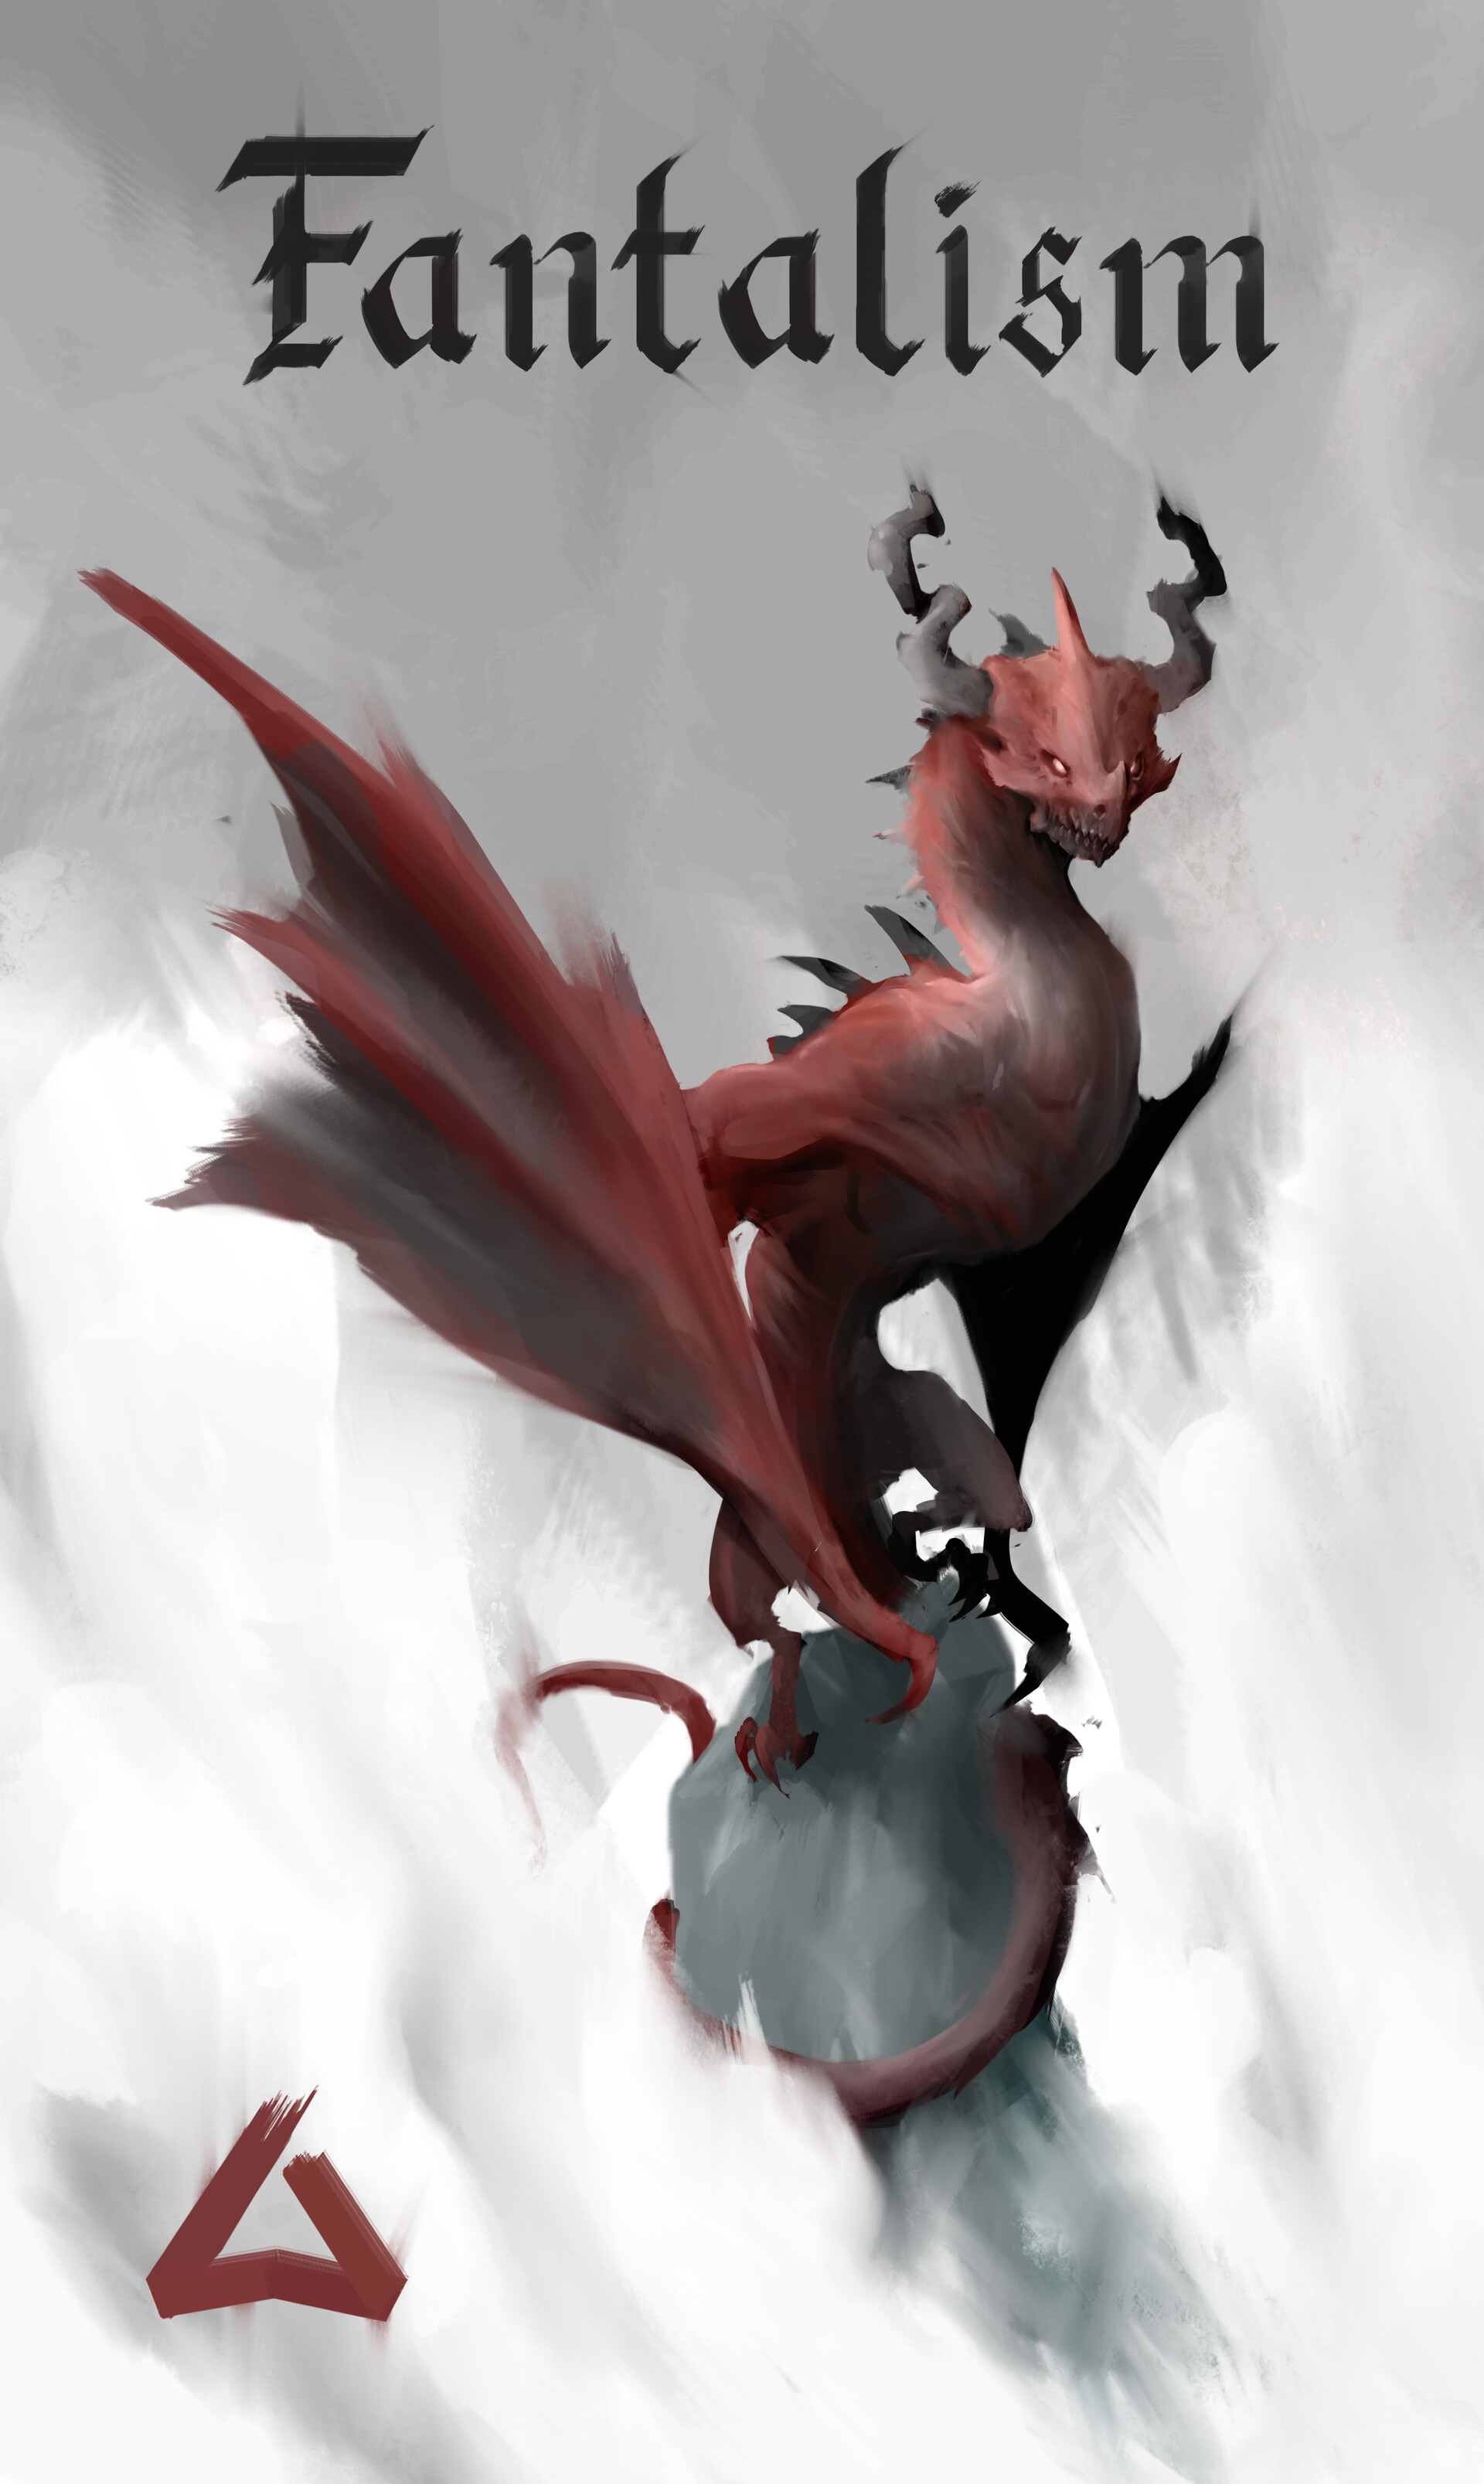
\includegraphics[width=50mm,scale=0.5]{img/arnesson-art-fantalism.jpg}
	\centering
	\caption{Fantalism: de webcomic van Arnesson Art, Thomas hugo.}
	\label{fig:fantalism}
\end{figure}
Thomas vertelde dat hij Reddit niet ziet als een ideaal medium voor te groeien. Het is als bedrijf moeilijk om deze kanalen goed te gebruiken. Als freelancer of gemotiveerde artist is dit veel toegankelijker, men wordt beter ontvangen op het platform.
	
\textbf{Wat zijn uw belangrijkste resources voor de groei van een bedrijf? Steunt u op AdWords, Facebook Ads etc?}
	
Voor Fantalism heeft Thomas Facebook Ads geprobeerd voor enkele tientallen euro's. Voor Thomas werkte dit echter niet zo goed, de interacties (lees: likes) die hij kreeg waren nutteloos. Ze deden dit enkel voor één post en hadden daarna geen interacties met nieuwe posts. Het was voor hem dus niet de moeite waard en het bleek dus moeilijk om op die basis een community uit te bouwen. Vandaar dat hij de aanpak behoudt van het posten op de juiste plaatsen, waar mensen interesse zouden tonen omdat ze het onderwerp heel leuk vinden. Die interacties zijn veel meer waard.

Thomas ziet dit voor Kriket ook niet direct als dé manier. Hij stelt voor om gratis samples uit te delen op plaatsen waar de doelgroep van Kriket zit, zoals campussen van hoge scholen of universiteiten. Mensen die bewust zijn van de milieuproblematiek, die openstaan voor iets nieuws en die bezig zijn met hun gezondheid.
	
\textbf{Heeft u ervaring met Zero Budget Marketing? Wat is hierbij het belangrijkste onderdeel van marketing?}
	
Tijdens Thomas zijn opleiding in Sint Lukas werden er enkele keren opdrachten gegeven omtrent marketing. Toen gaven de docenten de opdracht om het met zo weinig mogelijk budget (zero budget marketing) te doen. Dit was dus nooit of zelden het geval, vaak kwamen medestudenten af met ideeën uit guerillamarketing, zoals flyers uitdelen. Maar dan werd er niet gedacht aan ``Wie zal de flyers uitdelen\text{?}``, het antwoord was dan ``Studenten\text{?}``, ``En wie gaat die betalen\text{?}`` enzovoort... Het blijkt dus dat zero budget marketing zéér moeilijk is. Als je echt met geen of amper budget veel mensen wil bereiken moet je viraal gaan en dat is een grote uitdaging.
	
\textbf{Hoe ging u in het begin van uw carrière om met (community)-groei van een bedrijf en hoe doet u dat nu? Wat is er veranderd in die tijd? Wat heeft u geleerd?}
	
Thomas heeft voor zijn eigen bedrijf, Arnesson Art, ook moeten nadenken over groei. In eerste instantie was dit ``Hoe krijg ik opdrachten binnen\text{?}``. Zoals eerder vermeld heeft Thomas dit gedaan via Reddit. Hij heeft hieruit geleerd dat de directe aanpak goed werkt;

\begin{itemize} 
	\item ``Ik ben beschikbaar voor opdrachten``
	\item ``Hier is mijn portfolio``
	\item ``Ik werk enkel tegen betaling``
\end{itemize} 

Dat laatste is verrassend belangrijk, liet Thomas weten. Veel mensen verwachten vrijwilligerswerk of het delen van winst met een slecht idee, maar zo'n dingen betalen de huur van zijn appartement natuurlijk niet.

Toen werd er gevraagd ``Je vertelde eerder dat je niet geloofde in zero budget marketing en dat dit bijna altijd meer geld kost dan men verwacht, maar dit is toch zero budget marketing\text{?}``. Hierop antwoordde Thomas dat het niet gratis is, het kost nog steeds veel tijd om zo'n goede concrete, duidelijke en aantrekkelijke post te maken. Voordat deze op de juiste subreddit wordt gezet, wordt er veel tijd in gestoken om ze goed te maken. Deze tijd zou anders gebruikt kunnen worden om een opdracht uit te werken. ``Time is money``, ervaart hij zeer sterk sinds hij freelancer is.
	
\textbf{Waaruit bestaat een ideaal marketing team volgens u? In verhouding: hoeveel copywriters, digital marketeers, programmeurs, creatief ontwerpers, enz.?}
	
Een goed marketingteam opstellen is een hele grote klus volgens Thomas. Alle kwaliteiten dienen samen te komen uit verschillende functies, dit wil zeggen:

\begin{itemize} 
	\item Strateeg
	\item Copywriter
	\item Social media manager
	\item Creatief ontwerper
	\item Digital marketeer
	\item Programmeur of performance marketeer
\end{itemize} 

In een start-up zoals Kriket is het belangrijk dat het team zich verbonden voelt met het product. Het is bijna noodzakelijk dat je een passie hebt voor het product dat geproduceerd wordt.

Thomas vertelde dan het voor Kriket goed kan zijn om een nauwe samenwerking te starten met een klein digitaal marketingbureau, waarbij het bedrijf gemotiveerd is om samen met Kriket te groeien. De communicatie met het bureau is dan zeker belangrijk, dus er moet goed over nagedacht worden wie deze taak zal uitvoeren.
	
\textbf{Hoe belangrijk is viraal gaan voor een bedrijf? Is dit volgens u waar iedere marketeer, zoals uzelf, naar streeft? Of is het een specifiek doel dat op de juiste moment wordt achtervolgd?}
	
Waarschijnlijk streven veel marketeers naar een virale post op sociale media, maar dit is niet altijd wat de klant wil. Wanneer de klant bijvoorbeeld 5000 verkopen wil realiseren, kan het zijn dat een virale post voor maar 300 verkopen kan zorgen. Viraal betekent niet per sé goed, dit is wat veel mensen fout begrijpen. Wanneer de doelgroep niet juist zit heeft een video met 50 miljoen weergaven niet veel extra meerwaarde voor het bedrijf tegenover een video met 5000 weergaven.

Een goed voorbeeld hiervan is de video van Telenet die de nieuwe zender TNT had gelanceerd: ``Push to add drama``. Die video heeft nu meer dan 56 miljoen weergaven op TNT. Ondanks deze virale video heeft de zender TNT het maar ongeveer 1 jaar volgehouden. De video werd overal gedeeld, ook in het buitenland, maar daar heeft de zender helemaal geen baat bij. Met dit voorbeeld kan je vaststellen dat viraliteit absoluut geen garantie is voor succes.

Wat je wél wilt is mond tot mond reclame creëren, waar men tegen elkaar enthousiast over het product vertelt.

\textbf{Bij growth hacking spreekt men vaak over 2 à 3 belangrijke onderdelen: Creativiteit, Experimenteren/Analyseren van data en tot slot het Automatiseren en toepassen op technisch vlak. Ook bent u niet bewust bezig met growth hacking, deze onderdelen komen ook aan bod bij traditionele of digitale marketing.}
\begin{enumerate}[label*=\arabic*.]
	\item \textbf{Creativiteit: Hoe gaat u om met het creatieve proces van marketing? Bijvoorbeeld: Zijn hier brainstorm sessies voorzien? Heeft u creatieve ontwerpers die helpen?}
	
	Ten eerste is niet alle marketing creatief, dus het creatieve proces kan heel eenvoudig of onbestaande zijn. Bij dit soort marketing is het belangrijkste een goed design, de copy\footnote{De term ``copy`` wordt vaak gebruikt in deze branche om de tekst aan te duiden die (vaak) door een copywriter is geschreven.} is niet per sé creatief en kan eventueel gekopieerd worden van vroeger. Een goed voorbeeld is de solden periode, er zijn studies geweest over welke afbeelding en welke copy er werkt, dus die gebruiken de (grote) bedrijven. De bedoeling is dan gewoon om deze campagnes zo hard te pushen en te verspreiden dat iedereen ze gezien heeft, ze moeten helemaal niet creatief zijn.
	
	``Maar wat is dan wél creatieve marketing\text{?}``, dat is enerzijds een goede boodschap (copy) en een mooi en duidelijk beeld. Anderzijds is dit een goede strategische aanpak, bijvoorbeeld een partnership of een originele actie die er aan gekoppeld is.
	
	Een voorbeeld dat Thomas aanhaalde voor Kriket was als eerste een mooi beeld. Bijvoorbeeld een witte kast met een mooie groene plant bovenop, waarbij bladeren en stengels die naar beneden hangen. De kast ligt vol met Kriket bars die duidelijk gepresenteerd worden. Rond de kast zijn er echte krekels aanwezig voor het kleine ``shock``-effect. Naast deze foto kan men er ook een spel toevoegen aan deze marketingcampagne. Het spel kan via een mobiele applicatie of de Kriket website gespeeld worden. Het kan iets heel eenvoudig zijn in verband met krekels, waarbij de winnaar gratis Krikets ontvangt voor een aantal maanden.
	
	Bedrijven moeten durven en ook niet lui zijn, want dat is waar veel grote bedrijven de fout maken. Als men niet durft én lui is komt men terecht op de zoveelste saaie, niet-creatieve marketing post of campagne.
	
	\item \textbf{Data: Welke tools gebruikt u om informatie te verzamelen over uw doelpubliek? Welke tool is het belangrijkst en waarom?}
	
	Data verzamelen is de dag van vandaag zo makkelijk en uiteraard verschrikkelijk belangrijk, zeker wanneer men viraal gaat als bedrijf. Het belang van data is groot, maar het is wel dubbel.
	Men moet de data laten spreken, bijvoorbeeld bij een A/B-test\footnote{Bij A/B testen worden twee opties vergeleken bij een groep mensen, ieder krijgt ofwel A ofwel B en de conversies worden gebruikt als meetstaaf.}. Maar men moet niet verblind worden door de data, het grote geheel moet steeds bekeken worden. Soms zijn er andere factoren die de data hebben beïnvloed en die moeten natuurlijk worden meegenomen in het verhaal.
	
	Emotie is bijvoorbeeld iets dat moeilijk vatbaar is of ``brand awareness``, dit is niet makkelijk om te meten. Dit is duidelijk bij GDN (Google Display Network) banners. Wanneer men puur naar de cijfers kijkt, zijn GDN banners helemaal niet winstgevend. Hierbij moet men denken aan een groot reclamebord, dat is ook niet meteen winstgevend, maar het zorgt ervoor dat mensen het bedrijf leren kennen. Zo'n banners of reclameborden blijven de mensen wel bij en kan later, indirect, invloed hebben op de verkoop.
	
	\item \textbf{Automatiseren: Welke rol speelt IT of het IT-team bij marketing volgens u? }
	
	IT is niet meer weg te denken uit de marketing wereld. Tegenwoordig is het belangrijk voor de webmaster en marketeers om hun bij te scholen dat ze deze tools kunnen gebruiken, want ze worden heel uitgebreid. Men kan zelfs niet-creatieve marketing campagnes min of meer gaan automatiseren via deze tools. 
	
\end{enumerate}
\textbf{Growth hacking is vooral gekend bij online start-ups zoals Airbnb, Hotmail en Dropbox. Veranderd er volgens u veel bij growth hacking wanneer het niet meer gaat om een online bedrijf, maar wel een start-up met een fysiek product, zoals de krekelreep van Kriket?}

Dat kan natuurlijk, het moet niet per sé helemaal digitaal zijn. Ze kunnen natuurlijk wel die boeg uitslaan, als ze er volledig in geloven. Enkele voorbeelden van deze digitale aanpak zijn: Hello Fresh, Dollar Shave Club (VS), ... Deze bedrijven spelen enorm veel in op podcasts, influencers op sociale media zoals YouTube en referral-programma's. 

Kriket zou ook een abonnement-formule kunnen uitbrengen waarbij je iedere maand ofwel een ``mystery-box`` ontvangt ofwel een aantal krekelrepen dat je zelf kiest en eenvoudig kan aanpassen op ieder moment in de maand.


